% !TeX spellcheck = en_US
\newpage
\section{Wupper package}

In this section, the firmware, drivers, and tools of Wupper (see Figure~\ref{fig:simplewupperpackage}) together with its working principle are explained. For more detailed information about the internals and the core please refer to the official Wupper documentation~\cite{wupperoffical}.

\begin{figure}[h]
	\centering
	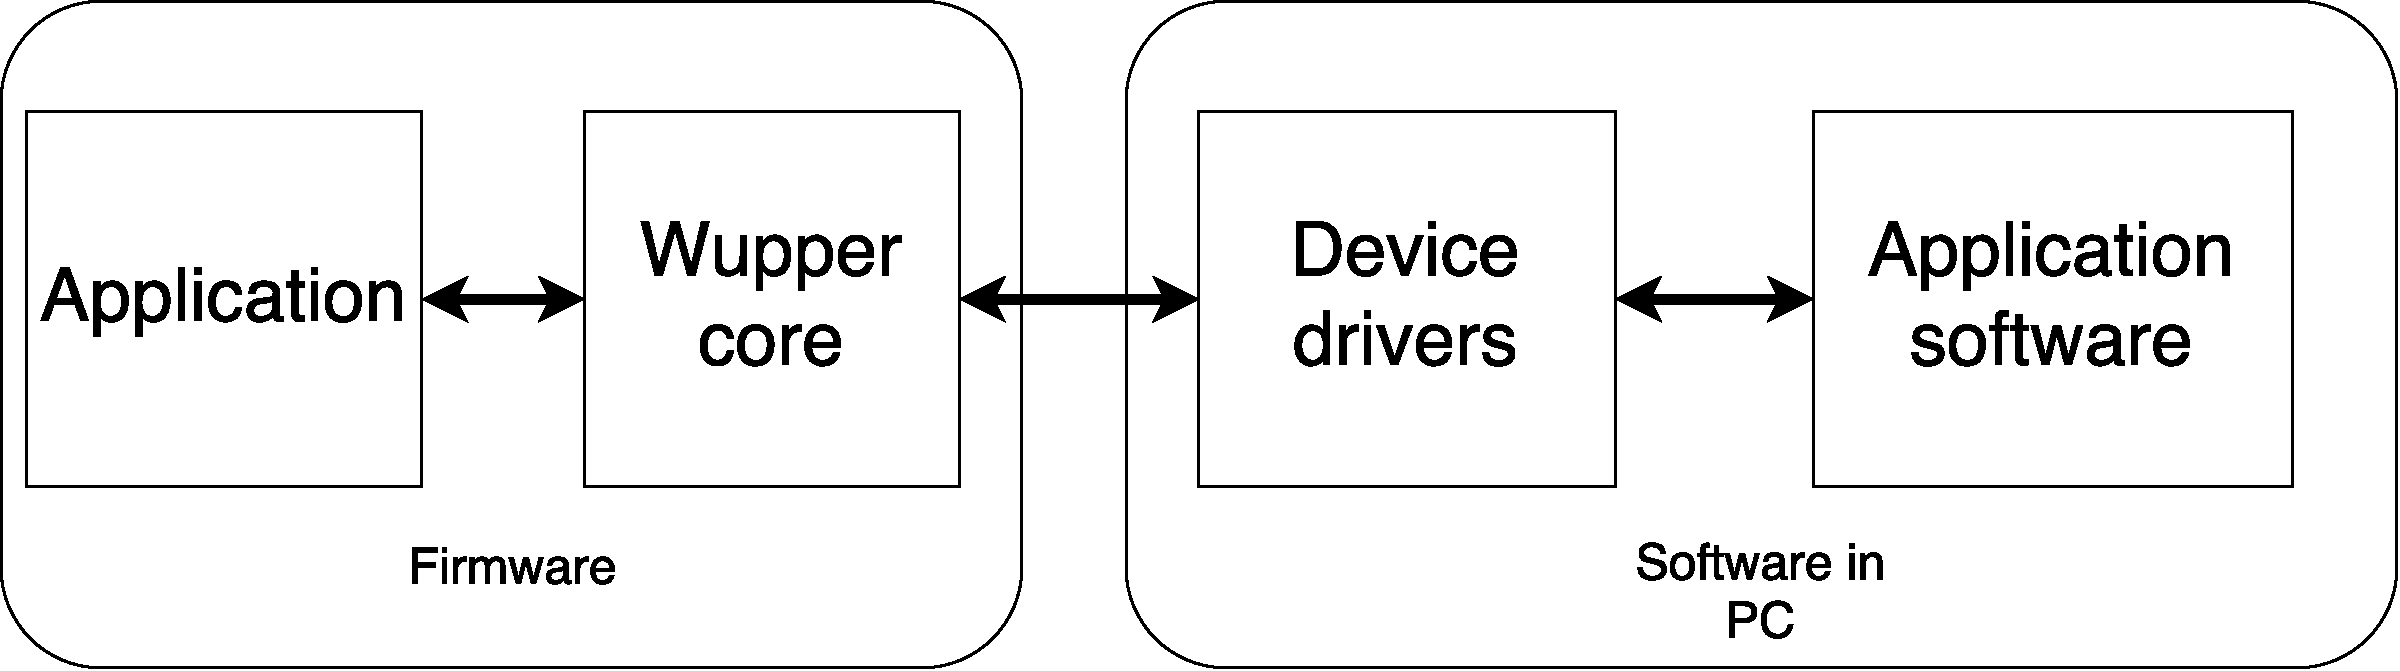
\includegraphics[width = .8 \textwidth]{figures/wupper_package_simple.pdf}	
	\caption{Wupper package overview}
	\label{fig:simplewupperpackage}
\end{figure}

\subsection {Wupper core}

%\begin{wrapfigure}[15]{r}{0.7\textwidth}
%	\centering
%	\vspace{-4mm}
%	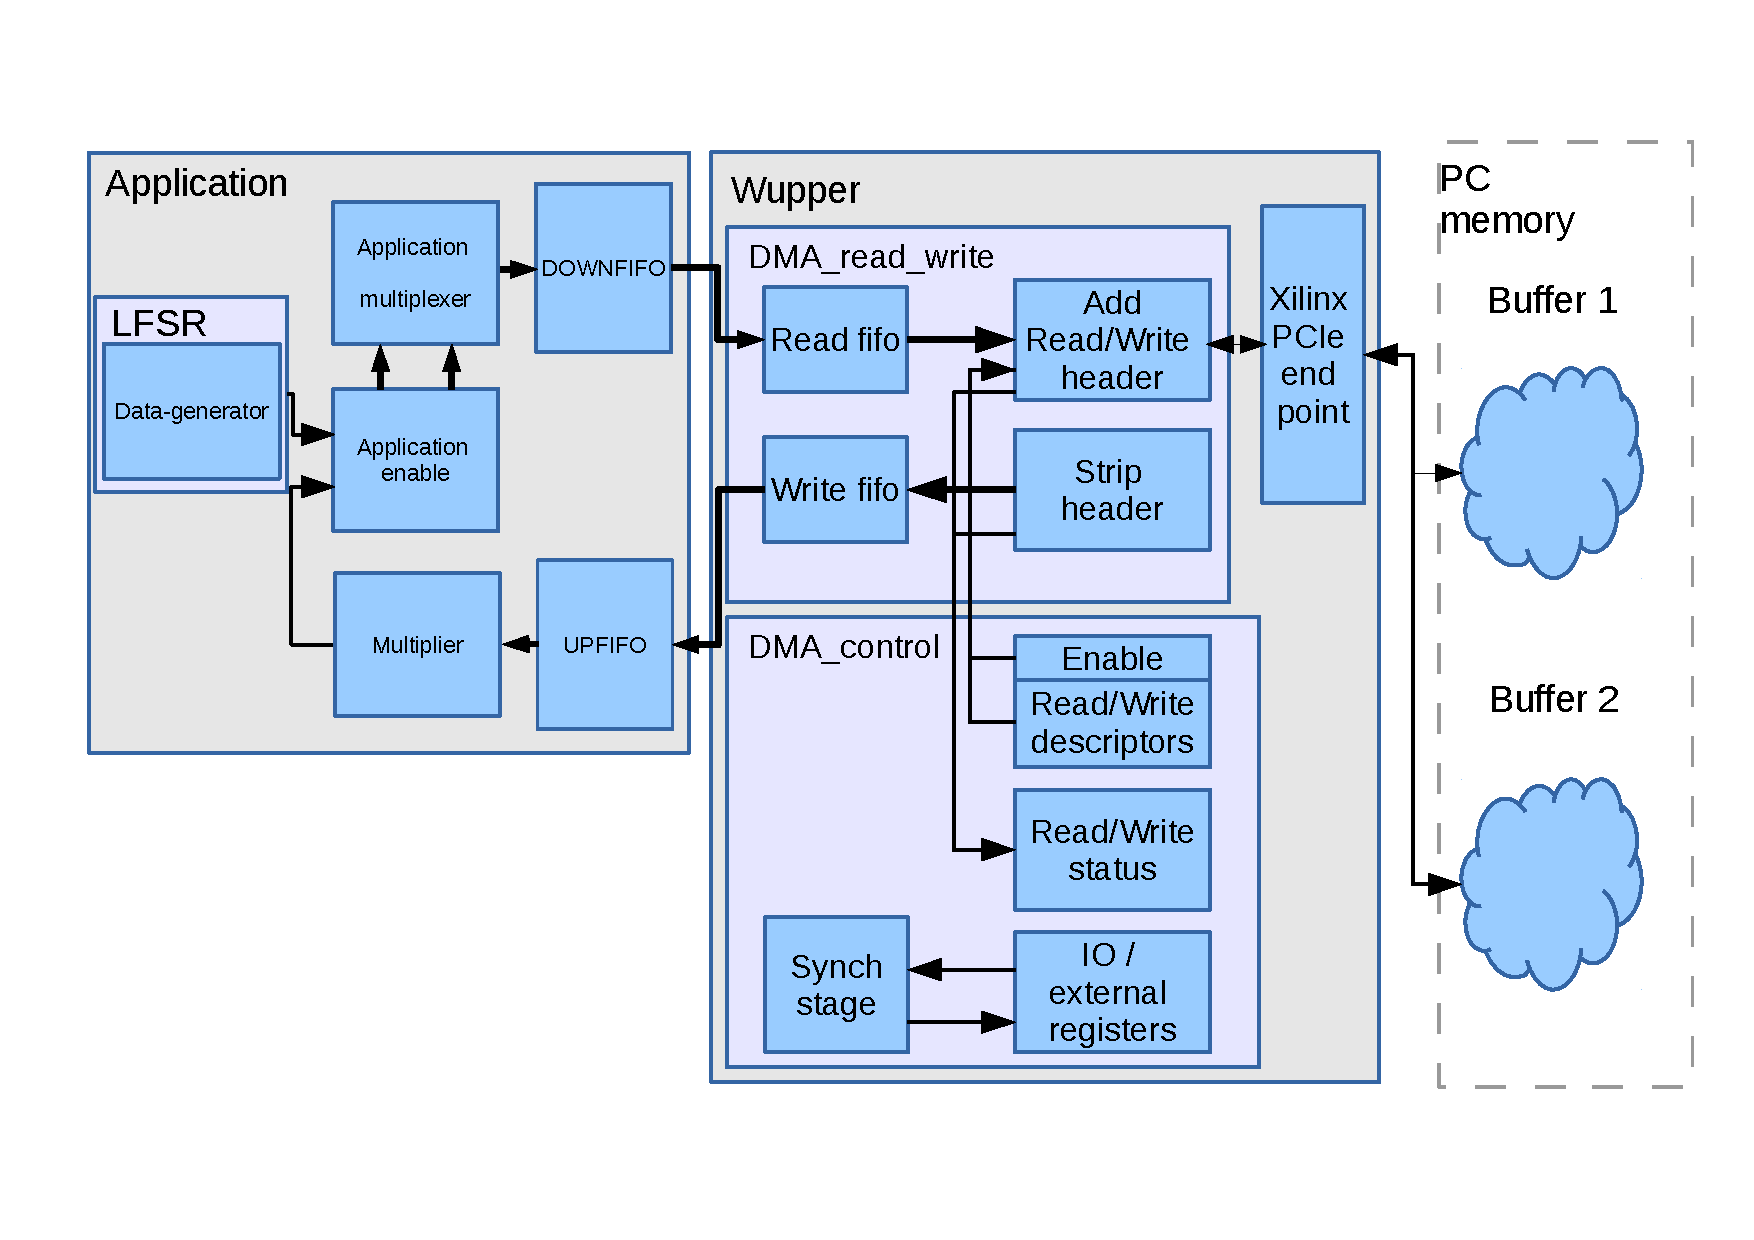
\includegraphics[width = 0.5 \textwidth]{figures/full_application_structure.pdf}	
%	\vspace{-3mm}
%	\caption{Overview of the HDL modules in the Wupper package}
%	\label{fig:wupperpackage}
%\end{wrapfigure} 

An Engine, like Wupper, moves data bidirectionally to a memory without CPU intervention. This efficient method is used for handling large amounts of data, which is crucial for throughput intensive applications. During a DMA tranfer, the DMA control core will take control according to the information provided by a DMA descriptor, and by flagging completion of operations in a per descriptor status register. By providing user data into the FIFO's, the core starts the DMA transfer over the PCIe lanes. Figure~\ref{fig:wupperpackage} shows a complete diagram of the of the HDL modules of the Wupper package; including the HDL modules for the Wupper core and the example application, together with the host PC memory.

\begin{figure}[h]
	\centering
	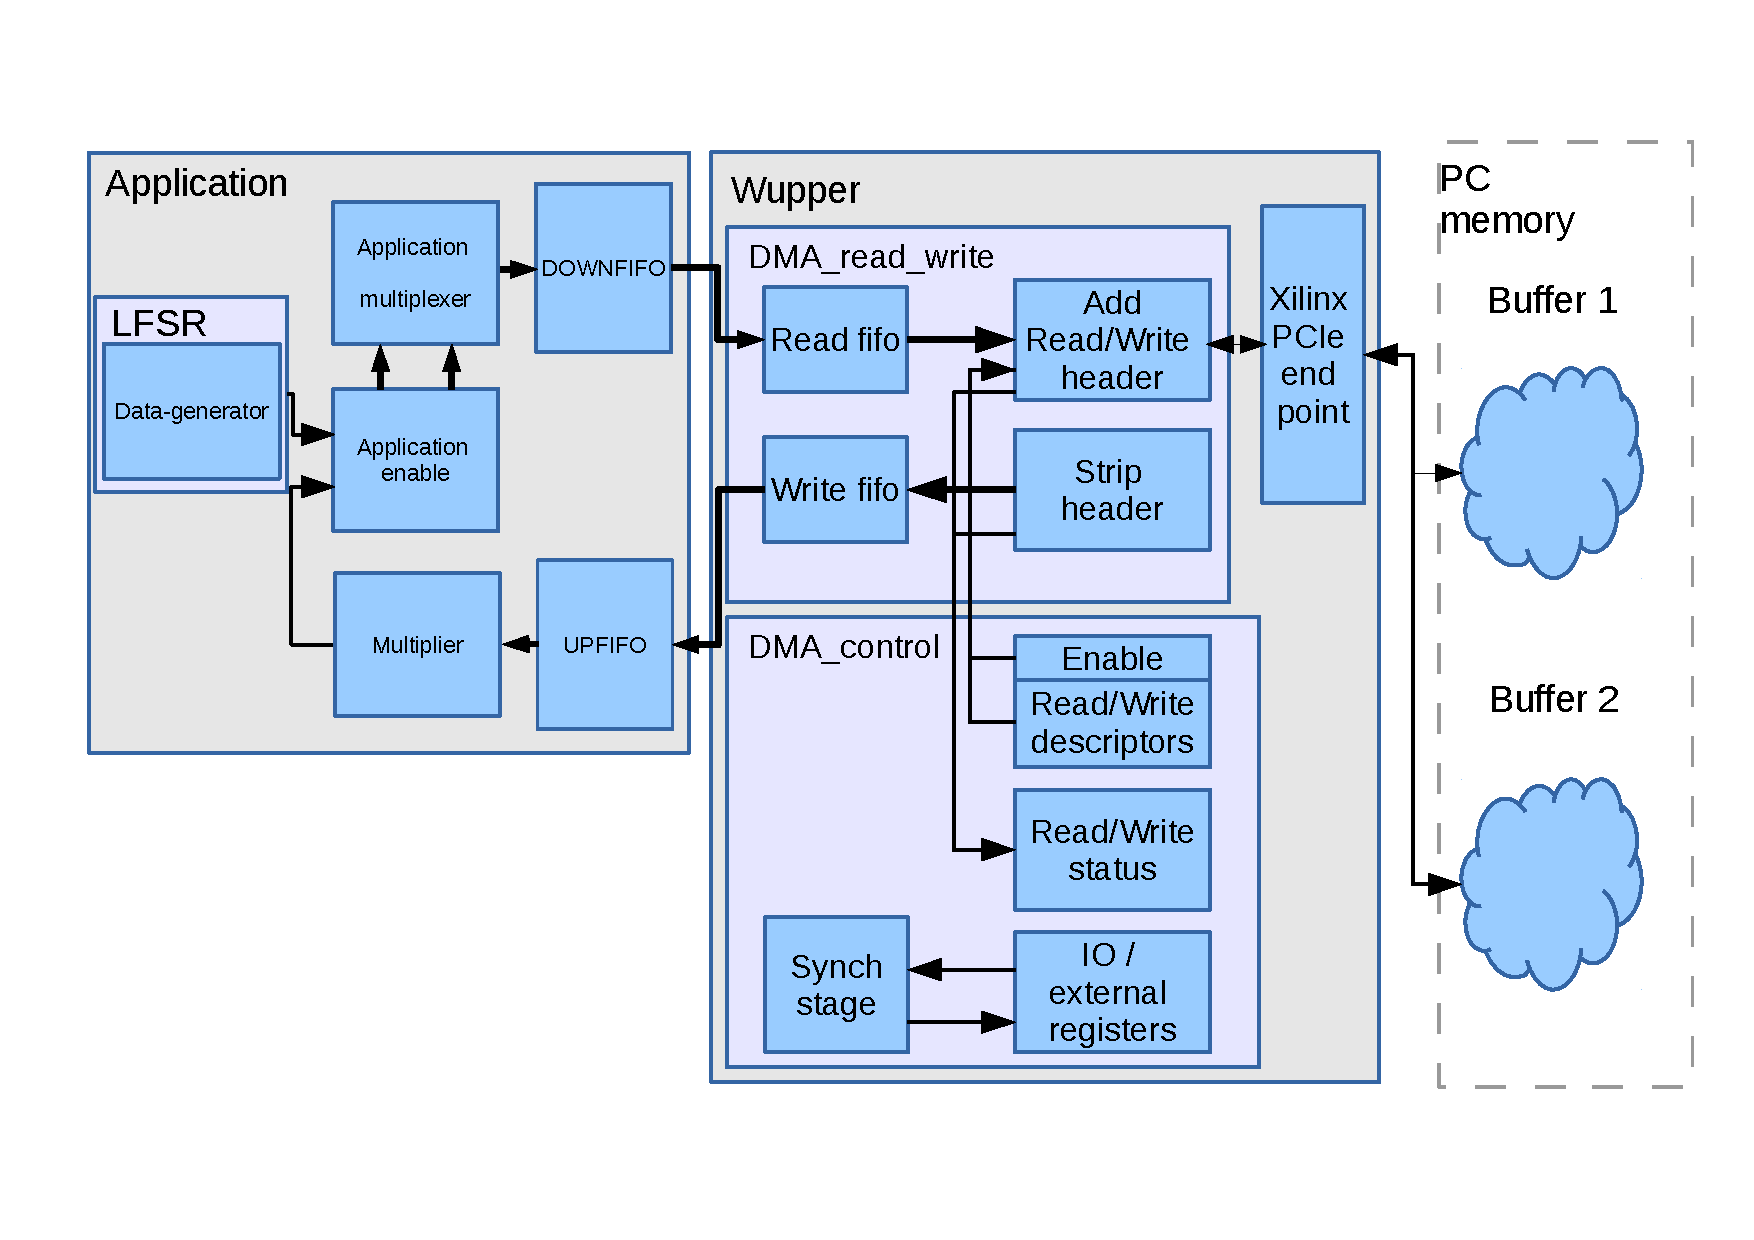
\includegraphics[width = 0.8 \textwidth]{figures/full_application_structure.pdf}	
	\caption{Overview of the HDL modules in the Wupper package}
	\label{fig:wupperpackage}
\end{figure}

% http://www.techonline.com/electrical-engineers/education-training/tech-papers/4370633/Introduction-to-DMA/viewpdf
% http://www.techonline.com/electrical-engineers/education-training/tech-papers/4136585/Universal-DMA-Controller-One-stop-solution-for-increasing-throughput-and-decreasing-latency-by-bypassing-CPU/viewpdf

\subsubsection {Xilinx PCIe End Point}


The Virtex-7 XC7VX690T-2FFG1761C on the VC-709 board has an integrated endpoint for PCI Express Gen3~\cite{pg023}. This black box handles the traffic over the PCI Express bus. Inside the Wupper core a DMA read/write process, sends and receives AXI4 commands over the AXI4-Stream bus. The black box translates this into differential electrical signals. Figure~\ref{fig:pciexpressendpoint} shows a simplified model of the firmware stack. Configuration of the core is explained in section 3.2 of the official documentation of Wupper~\cite{configpciecore}.

\begin{figure}[h]
	\centering
	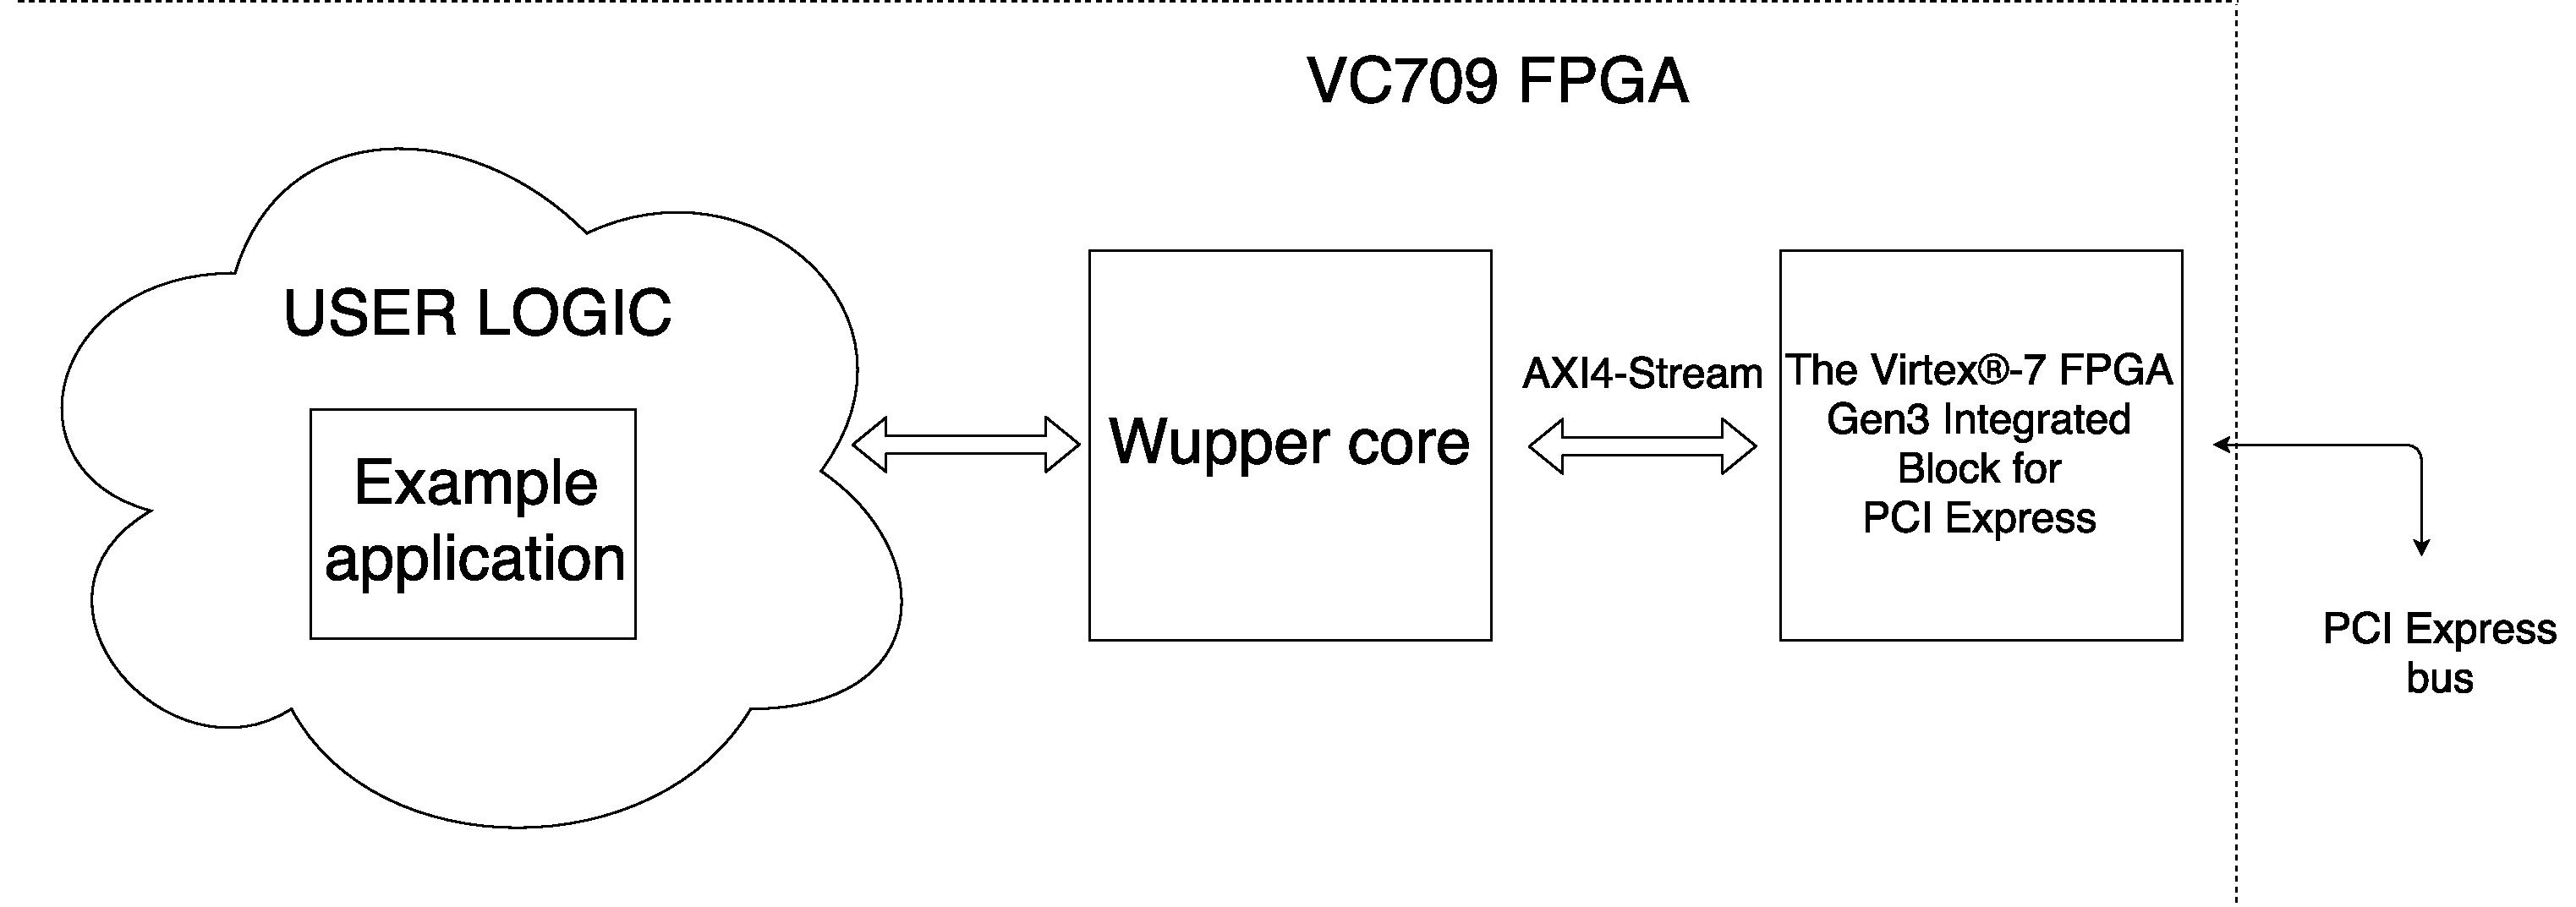
\includegraphics[width = 1 \textwidth]{figures/PG023.pdf}	
	\caption{Block diagram of the logic in the VC-709 FPGA}
	\label{fig:pciexpressendpoint}
\end{figure}

\subsubsection {Core control} 
The DMA control (DMA\_control in Figure~\ref{fig:wupperpackage}) process consists of a register map which can be configured from a PC using the Wupper tools. The registermap is divided in three regions: BAR0, BAR1 and BAR2. BAR stands for Base Address Region. Every BAR has 1 MB of address space.

BAR0 contains registers associated with DMA like the DMA descriptors. The descriptors specify the addresses, transfer direction, size of the data and an enable line. Figure~\ref{fig:wupperpackage} shows that the information is fed to the DMA\_read\_write core.

BAR1 is reserved for the interrupt mechanism and consists of 8 vectors.

BAR2 is used for the benchmark application and is dedicated to user applications. The work done for this report defines and acts on registers in BAR2, as summarized in Appendix ~\ref{sec:bar2}. 



 As previously shown in Figure~\ref{fig:wupperpackage}, the example application core consists of multiple function blocks which are attached to the register map. This makes it possible to control the benchmark application from the PC. 
A complete overview of the register map can be found in the official documentation of Wupper ~\cite{wupperoffical}.




%The content related to the benchmark application will be discussed in the section   


%The DMA control process consist of two Read / Write subprocesses: descriptors and status. The descriptors are parsed in the Read / Write descriptors process 
\newpage
\subsubsection {DMA read/write}
The DMA read and write (DMA\_read\_write in Figure~\ref{fig:wupperpackage}) module handles the transfer from the FIFO's according to the direction specified by the descriptors. If data shifts into the down FIFO, a non-empty flag will be asserted to start the DMA write process, this direction of the flow is defined as the "down link". This process reads the descriptors and creates a header with the information. The header is added when the data shifts out of the down FIFO. For the reversed situation, the data with a header is read from the PC memory. This direction of the flow is then defined as "up link". The information in the header will be parsed by the DMA control and the data fed to the up FIFO.




\subsection{Example application HDL modules}
The example application, the user application inside the FPGA, replaces the counter with a pseudo-random data generator. Moreover the new feature in the application has the possibility to process data from the PC memory. The example application can be operated in two modes:

\begin{enumerate}
	\item The random data generator directly sends data to the host via Wupper, this is referred to as "write only" or "half loop" test. 
	\item The content of the random data generator is wrote back to the FPGA, multiplied and sent to host again, this is referred as "read and write" or "full loop" test.  
	
\end{enumerate}

The example application is developed in VHDL, and the code is synthesized and implemented in Xilinx Vivado 2014.4~\cite{vivadoman}. The example application is now part of the Wupper package on OpenCores. 

\subsubsection {Functional blocks}

Figure~\ref{fig:benchmarkapp} shows a detailed block diagram of the example application for Wupper. The Wupper core contains a list of addresses, this list is the register map. The values of the register map are implemented in the firmware as signals. The PC sees the signals as addresses. Wupper tools write values to these addresses which control the FPGA logic (see dashed lines in Figure~\ref{fig:benchmarkapp}).
%http://www.eetimes.com/document.asp?doc_id=1274550

\begin{figure}[h]
	\centering
	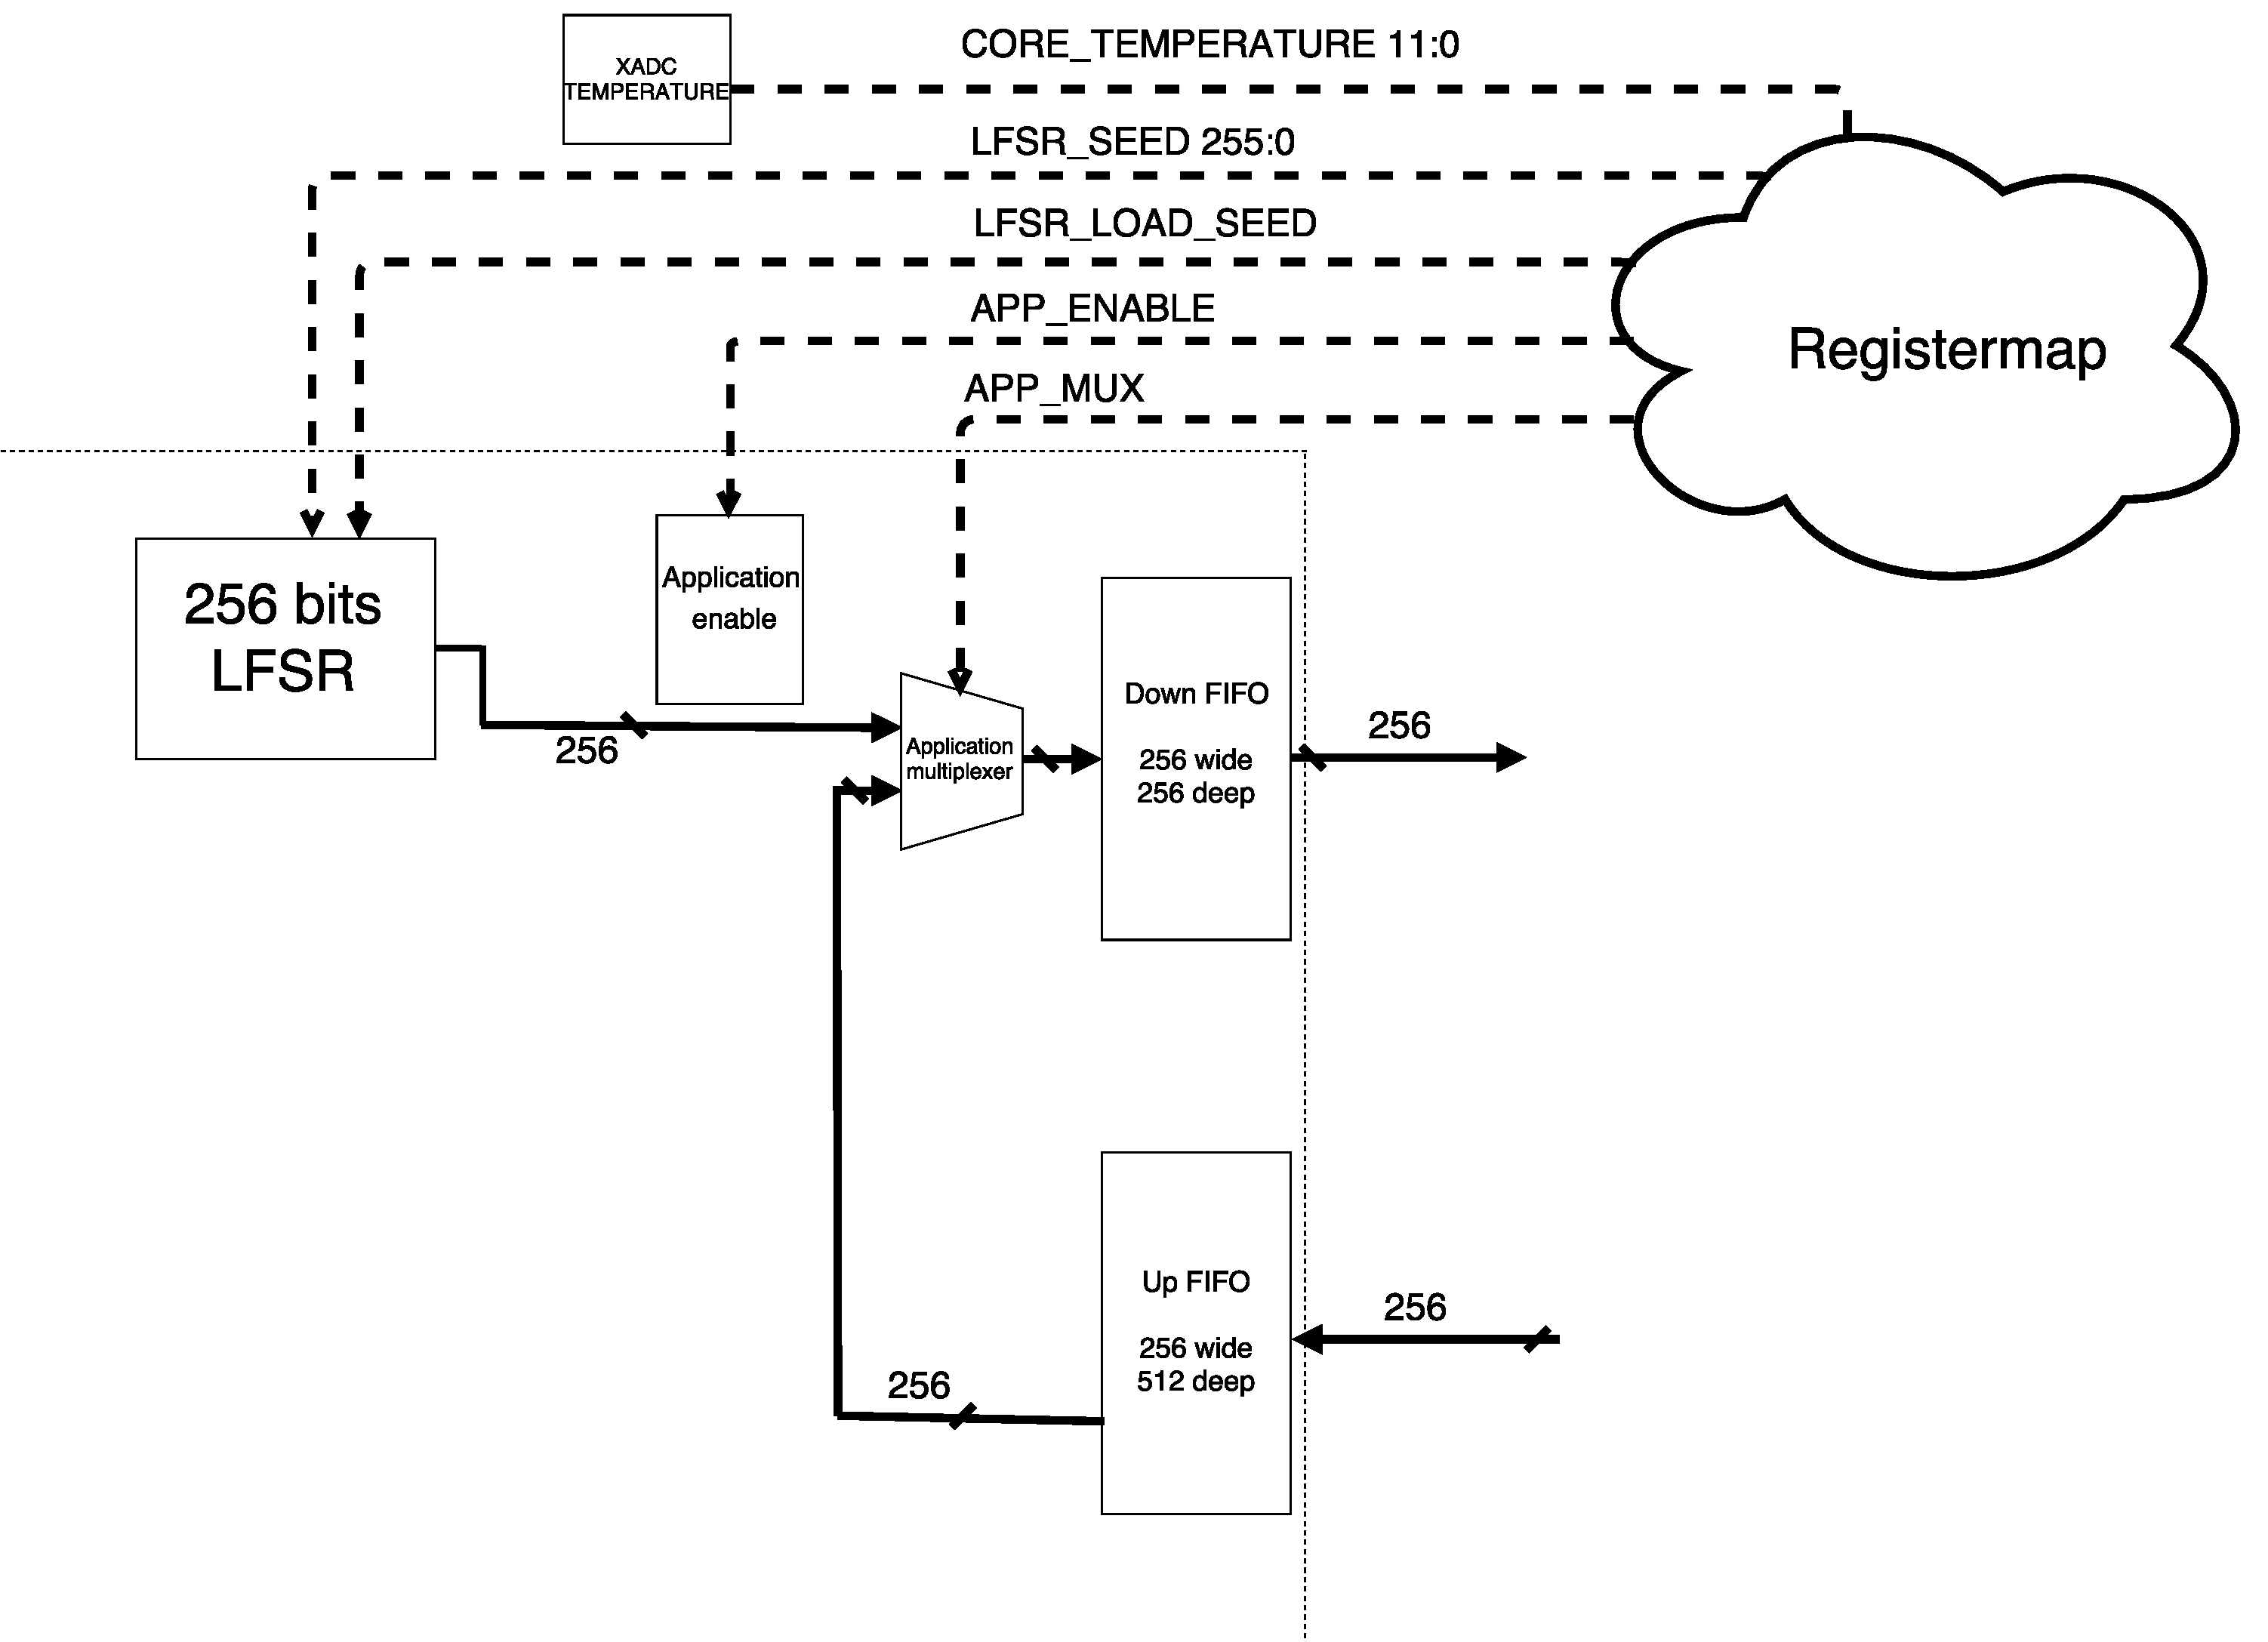
\includegraphics[width = 0.8 \textwidth]{figures/benchmark_application.pdf}	
	\caption{Overview of the example application}
	\label{fig:benchmarkapp}
\end{figure}

\newpage
As introduced in the previous paragraph, one type of test possible with the example application is the "half loop": in such mode of operation, Wupper is fed by a random data generator based on a 256 bits Linear Feedback Shift Register (LFSR). An LFSR, as shown in Figure~\cite{lfsr}, consists of a number of shift registers which are fed back to the input. The feedback is manipulated by an XOR operation which creates a pseudo-random pattern. The ideal goal is to produce a sequence with a infinite length to prevent repetition. Repetition occurs by two factors, the feedback points/taps and the start value. The maximal length sequence can be approached by $2^n-1$~\cite{lfsr}. Where the $n$ is the number of shift registers. The 256 bits LFSR is a four stage Galois LFSR with taps at the registers 256, 254,251 and 246. The approach is explained in paper~\cite{lfsrtable} by R. W. Ward and T.C.A. Molteno of the electronics group at the University of Otago.
The software tools developed for the example application initialize the seed value by writing it to the register map thereafter the 1-bit $LFSR\_LOAD\_SEED$ signal is set to 1. This resets the LFSR process with a seed value.

\begin{figure}[h]
	\centering
	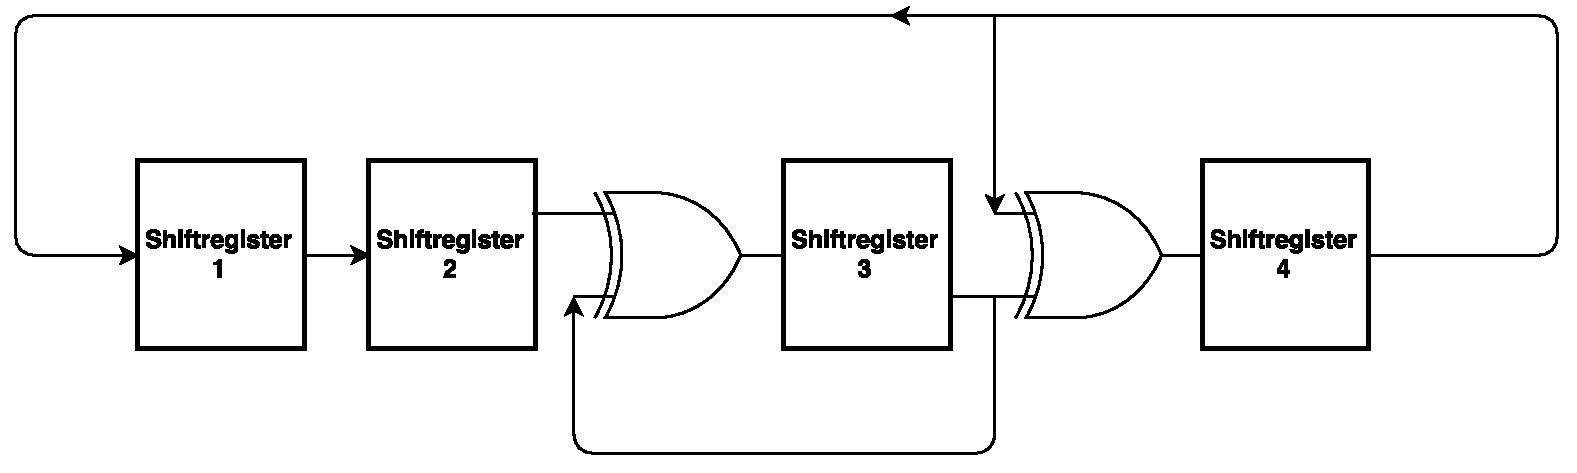
\includegraphics[width = 0.8 \textwidth]{figures/lfsr.pdf}	
	\caption{A 4 bit Linear Feedback Shift Register (LFSR)}
	\label{fig:lfsr}
\end{figure}
%http://www.newwaveinstruments.com/resources/articles/m_sequence_linear_feedback_shift_register_lfsr.htm
\newpage
For the full loop example, the two fifos are simply connected to each other. This way a full duplex PCIe dma can be performed.

For monitoring the core temperature, a XADC IP block~\cite{xadc} is used. This is generated by Vivado's XADC wizard. The output signal of the block is connected to one register of the register map.

The 1-bit signal $APP\_MUX$ is attached to the select port of the application multiplexer. This enables the data flow to the down FIFO.

The signal $APP\_ENABLE$ enables the output of the LFSR and the fromhost fifo. 

The FIFO's are generated by Vivado's FIFO generator and using integrated common clock block RAMs. The clock is set to 250 MHz to reach the maximum theoretical throughput. The up FIFO is deeper to function as a buffer. This is an extra precaution. The reason is if the data is looped back in the application, both FIFO's can be full at the same time. If this occurs, the application stalls because of the loop back.

\newpage


\subsection{Device driver and Wupper tools}


The Wupper tools communicate with the Wupper core through the Wupper device driver. Buffers in the host PC memory are used for bidirectional data transfers, this is done by a part of the driver called CMEM. This will reserve a chunk of contiguous memory in the host. For the specific case of the example application, the allocated memory will be logically subdivided in two buffers (buffer 1 and buffer 2 in Figure~\ref{fig:wupperpackage}). One buffer is used to store data coming from the FPGA (write buffer, buffer 1), the other to store the ones going to the FPGA (read buffer, buffer 2). The idea behind the logical split of the memory in buffers is that those buffers can be used to copy data from the write to read, and perform checks. The driver is developed for Scientific Linux CERN 6 but has been tested and used also under Ubuntu kernel version 3.13.0-44a. Building and loading/unloading the driver is explained in section 6.1.2 en 6.1.3 of the official documentation of Wupper~\cite{operatingpcieengine}.

The Wupper tools are a collection of tools which can be used to debug and control the Wupper core. These tools are command line programs and can only run if the device driver is loaded. A detailed list and explanation of each tool is given in the next paragraphs. Along with the collection of tools derived from the FELIX tool suite, the Wupper-dma-transfer and Wupper-chaintest had been added as new features for the OpenCores' benchmark. As mentioned before, the purpose of those applications is to check the health of the Wupper core. 

The Wupper tools collection comes with a readme~\cite{wupperreadme}, this explains how to compile and run the tools. Most of the tools have an -h option to provide helpful information. The table below shows a list of the tools derived from the original flxtools suite and their description.

\begin{center}
	\begin{tabular}{ | l || p{10cm} |}
		\hline
		Tool & Description                       \\ \hline

		Wupper-info
		&  Prints information of the device. For instance device ID, PLL lock status of the internal clock and FW version.
		\\ \hline
		
		Wupper-reset
		&  Resets parts of the example application core. These functions are also implemented in the Wupper-dma-transfer tool.
		\\ \hline
				
		
	    Wupper-config
		& Shows the PCIe configuration registers and allows to set, store and load configuration. An example is configuring the LED's on the VC-709 board by writing a hexadecimal value to the register.
                                     \\ \hline
  		Wupper-irq-test
  		&  Tool to test interrupt routines
  		\\ \hline
		
		Wupper-dma-test
		& This tool transfers every second 1024 Byte of data and dumps it to the screen.
	                                           \\ \hline
	
   		Wupper-throughput
   		&  The tool measures the throughput of the Wupper core. The method of computing the throughput is wrong, this is discussed in the section 3.4.2.
   		\\ \hline
	    		                                       
		
		Wupper-dump-blocks
		&  This tools dumps a block of 1 KB. The iteration is set standard on 100. This can be changed by adding a number after the "-n".
		                                          \\ \hline

	\end{tabular}
\end{center}

For the Wupper package on OpenCores two extra tools had been newly developed to target specific benchmark requirement for the generic example application: Wupper-dma-transfer and Wupper-chaintest. In the next paragraphs a detailed description of such tools and their operation is given.

\newpage

\subsubsection{Operating Wupper-dma-transfer}

Wupper-dma-transfer sends data to the target PC via Wupper also known as half loop test. This tool operates the benchmark application and has multiple options. A list of such options is summarized in Listing~\ref{lst:dmatoollist}.

\begin{lstlisting}[language=BASH, frame=single, label={lst:dmatoollist}, caption=Output of Wupper-dma-transfer -h]
daqmustud@gimone:$ ./wupper-dma-transfer -h

Usage: wupper-dma-transfer [OPTIONS]


This application has a sequence: 
1 -Start with dma reset(-d)
2 -Flush the FIFO's(-f)
3 -Then reset the application (-r)


Options:
-l             Load pre-programmed seed.
-q             Load and generate an unique seed.
-g             Generate data from PCIe to PC.
-b             Generate data from PC to PCIe.
-s             Show application register.
-r             Reset the application.
-f             Flush the FIFO's.
-d             Disable and reset the DMA controller.
-h             Display help.


\end{lstlisting}


 Before using the write function, make sure that the application is ready by resetting all the values, as shown in Listing~\ref{lst:dmatoolreset}.

\begin{lstlisting}[language=BASH, frame=single, label={lst:dmatoolreset},  caption=Reset Wupper before a DMA Write action]
daqmustud@gimone:$ ./wupper-dma-transfer -d
Resetting the DMA controller...DONE! 
daqmustud@gimone:$ ./wupper-dma-transfer -f
Flushing the FIFO's...DONE! 
daqmustud@gimone:$ ./wupper-dma-transfer -r
resetting application...DONE! 
\end{lstlisting}

\newpage

\noindent
Before writing data into the PC, the data generator needs a seed to initialize the generator. There are two options available: load a unique seed or load a pre-programmed seed. The pre-programmed seed is always 256 bits, the unique seed value can be variable. The -s option displays the status of the register including the seed value. For a unique seed, replace the -l with -q, as shown in Listing~\ref{lst:dmatoolseed}.

\begin{lstlisting}[language=BASH, frame=single, label={lst:dmatoolseed}, caption=Loading a pre-programmed seed in to the data generator.]
daqmustud@gimone:$ ./wupper-dma-transfer -l
Writing seed to application register...DONE! 
daqmustud@gimone:$ ./wupper-dma-transfer -s

Status application registers
----------------------------
LFSR_SEED_0A:        DEADBEEFABCD0123 
LFSR_SEED_0B:        87613472FEDCABCD 
LFSR_SEED_1A:        DEADFACEABCD0123 
LFSR_SEED_1B:        12313472FEDCFFFF 
APP_MUX:             0 
LFSR_LOAD_SEED:      0
\end{lstlisting}


The -g option performs a DMA write to the PC memory. The data generator starts to fill the down FIFO and from the PC side, a DMA read action is performed. The size of the transfer is set to 1 MB by default, but the size is configurable. When the PC receives 1 MB of data, the transfer stops. It is possible that there is still some data left in the down FIFO, resetting the FIFO's can be done by the -f option, as shown in Listing~\ref{lst:dmatoolwrite}.

\begin{lstlisting}[language=BASH, frame=single, label={lst:dmatoolwrite}, caption=Start generating data to the target.]
daqmustud@gimone:$ ./wupper-dma-transfer -g
Starting DMA write
done DMA write 
Buffer 1 addresses:
0: EED9733362A50D71 
...
...
...
\end{lstlisting}

\newpage

In a similar way a DMA read action from the FPGA can be performed by using the -b option. The output of the up FIFO is fed to the loopback. The output of the loopback is fed to the down FIFO with a destination to the PC memory as shown in Listing~\ref{lst:dmatoolback}.

\begin{lstlisting}[language=BASH, frame=single, label={lst:dmatoolback}, caption= Performing a DMA read and DMA write]
daqmustud@gimone:$ ./wupper-dma-transfer -b
Reading data from buffer 1...
DONE!
Buffer 2 addresses:
0: 24BBEC63B53F3BCC 
...
...
...
\end{lstlisting}

\subsubsection{Operating Wupper-chaintest}
The Wupper-chaintest tool does in one shot a complete DMA Read and Write transfer. It checks if the loopback data is done correctly. This is done by comparing the output of the data in buffer 1 and 2 (shown earlier in Figure~\ref{fig:wupperpackage}). The tool returns the number of errors out of 65536 loops as shown in Listing~\ref{lst:chaintest}.
\begin{lstlisting}[language=BASH, frame=single, label={lst:chaintest}, caption=Output of Wupper-chaintest]
daqmustud@gimone:$ ./wupper-chaintest      
Reading data from buffer 1...
DONE!
Buffer 2 addresses:
0: 49A5A89745420D34 
...
...
... 
9: 5D37679AE79FA7C2 
0 errors out of 65536
\end{lstlisting}

\newpage


\subsection {Wupper GUI}

The concept of the Wupper GUI is based on the Wupper tools and has the same construction (see Figure~\ref{fig:softwaretree}). The GUI is developed with Qt version 5.5 (C++ based)~\cite{qt} and gives the user a visual feedback of the Wupper's status/health. The GUI can only run if the device driver is loaded.

\begin{figure}[h]
	\centering
	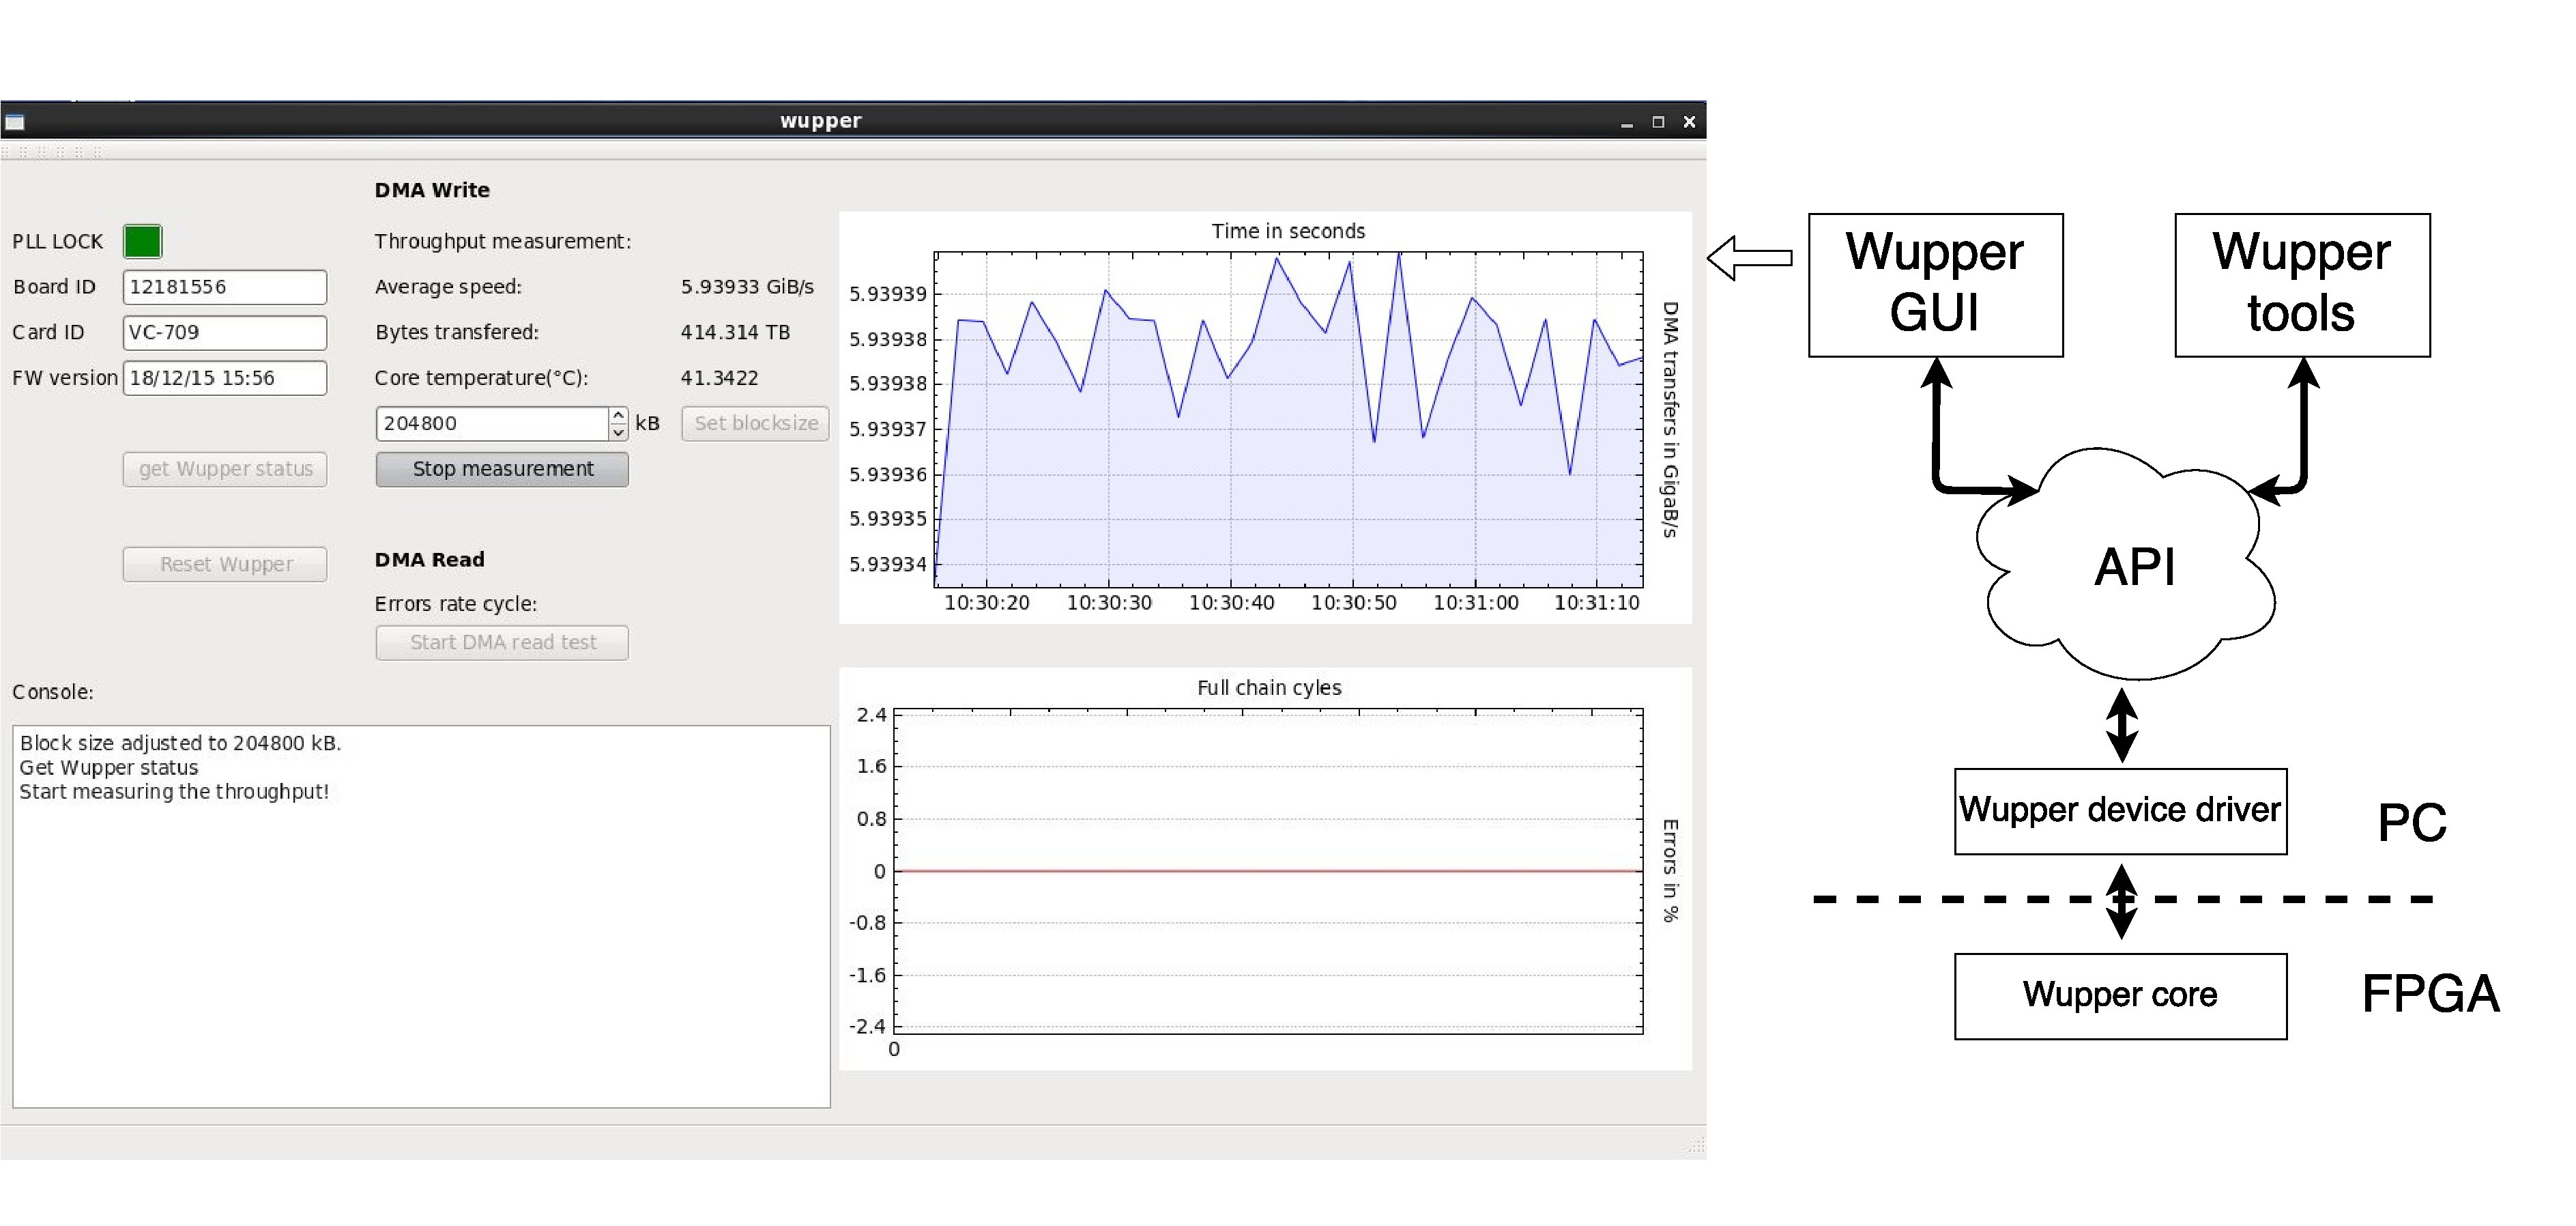
\includegraphics[width = 0.7 \textwidth]{figures/tree.pdf}	
	\caption{High and low level software overview block diagram.}
	\label{fig:softwaretree}
\end{figure}

\subsubsection {Functional blocks and threaded programming}


 Multi-threading is used so functional blocks can run at the same time as the GUI. If multi-threading is not used, the GUI interface gets stuck. A thread starts a new process next to the main process. If another processor core is available, the thread will run on a separated core. By communicating via slots to the main process, the data is secured.
There are two threads but only one of the threads can be used at the same time. The reason is that both threads use the same DMA ID, this will cause an error.
The threads communicate with the Application Program Interface (API) to control and fetch the output of the logic. The output data communicate safely via a signal to the slots. Figure~\ref{fig:guithreads} shows an overview of the threaded programs in the Wupper GUI.

\begin{figure}[h]
	\centering
	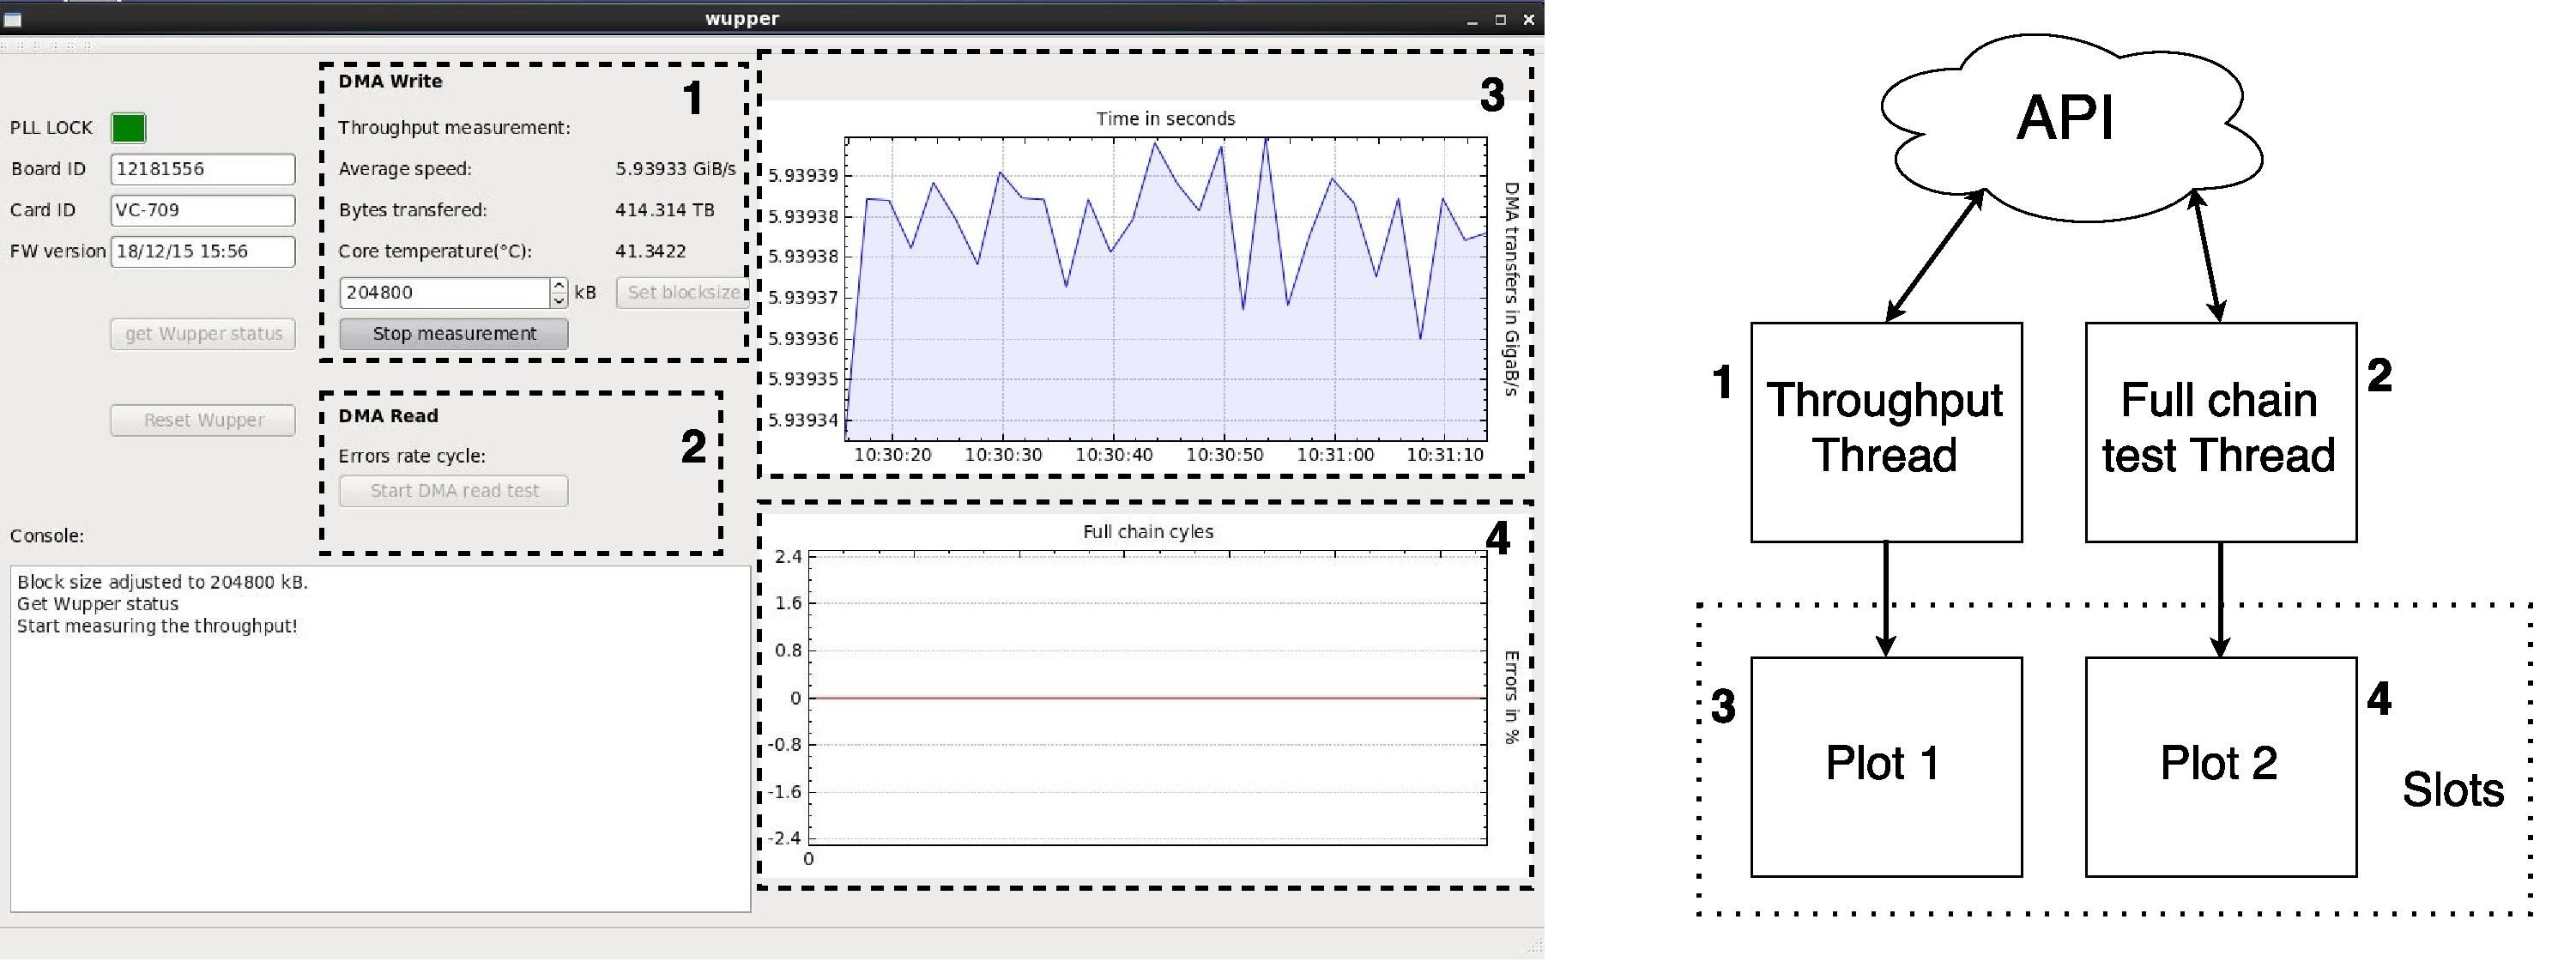
\includegraphics[width = 0.9 \textwidth]{figures/wupper_gui_threads_overview.pdf}	
	\caption{Threaded programs in the Wupper GUI}
	\label{fig:guithreads}
\end{figure}

\newpage
\subsubsection {GUI operation}

The GUI is separated in four regions (see Figure~\ref{fig:wuppergui}): status, control, measurement and an info region.
The status region fetches the information about various parts of the FPGA on the VC-709 via the Wupper core, and about the core itself. When the user clicks on the "get Wupper status" button, it shows the internal PLL lock status, Board ID, Card ID and the firmware version.

The control region controls the logic inside Wupper through the API. The "Reset Wupper" button resets the application logic by resetting the DMA, flushing the FIFO's and reset the application values. 

In the DMA Write section, the user can perform a DMA Write measurement. The user can configure the blocksize. The blocksize has effect on the speed, this is discussed in Appendix ~\ref{sec:blocksize}. The measurement output is shown in the measurement region. The method of computing the throughput is different than the method of the Wupper-throughput tool. The fault is the wrong order of operations by misplacing brackets. The wrong method is $A/B*C= D$ instead of $A/(B*C)= D$.

In a similar way, the user can perform a DMA Read test and the output is shown in the plot in the measurement region.
The info/console output region gives the user feedback of the application and the GUI.

\begin{figure}[h]
	\centering
	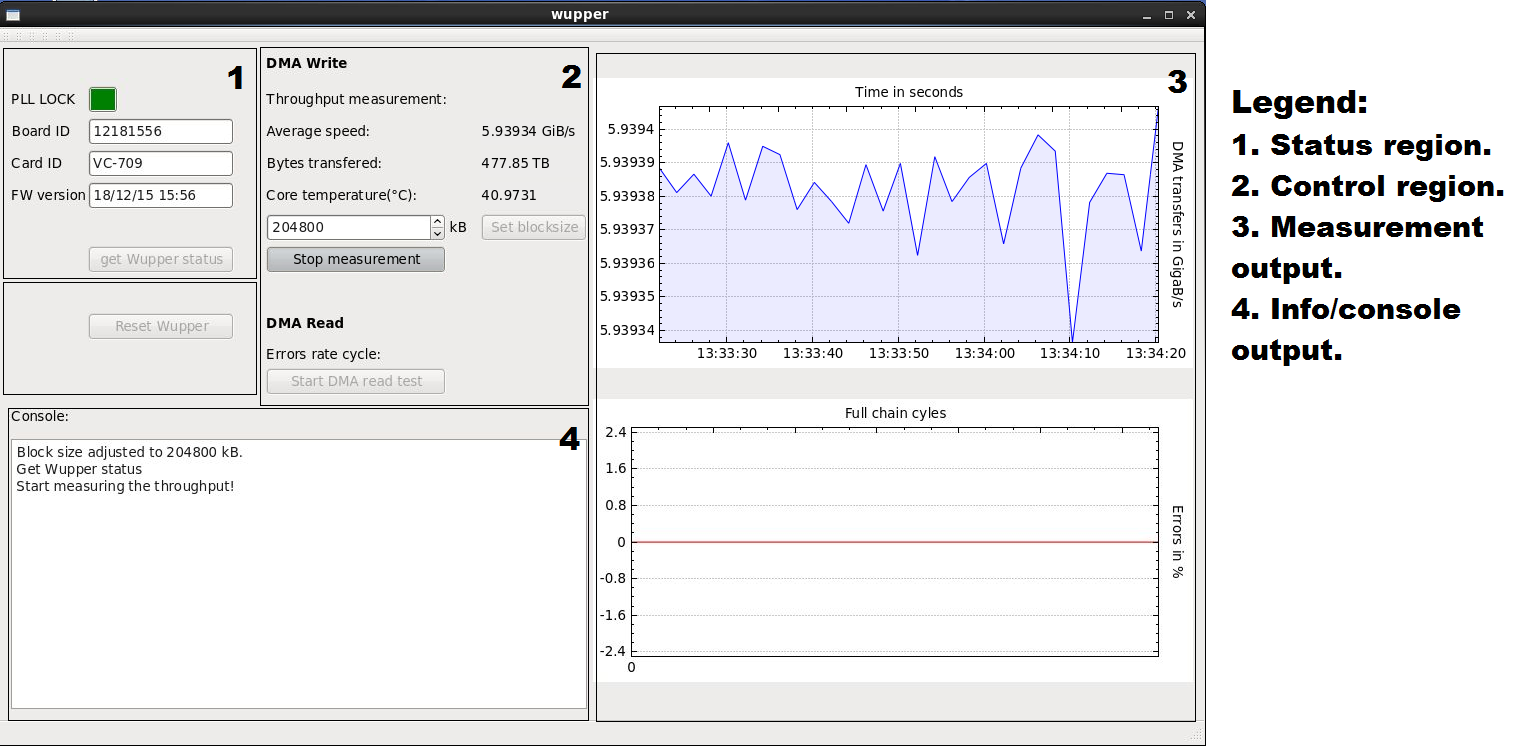
\includegraphics[width = 1 \textwidth]{figures/gui_printscreen_tb.PNG}	
	\caption{Screenshot of the example application GUI}
	\label{fig:wuppergui}
\end{figure}

 




\newpage










\newpage